
%%%%%%%%%%%%%%%%%%%%%%% file typeinst.tex %%%%%%%%%%%%%%%%%%%%%%%%%
%
% This is the LaTeX source for the instructions to authors using
% the LaTeX document class 'llncs.cls' for contributions to
% the Lecture Notes in Computer Sciences series.
% http://www.springer.com/lncs       Springer Heidelberg 2006/05/04
%
% It may be used as a template for your own input - copy it
% to a new file with a new name and use it as the basis
% for your article.
%
% NB: the document class 'llncs' has its own and detailed documentation, see
% ftp://ftp.springer.de/data/pubftp/pub/tex/latex/llncs/latex2e/llncsdoc.pdf
%
%%%%%%%%%%%%%%%%%%%%%%%%%%%%%%%%%%%%%%%%%%%%%%%%%%%%%%%%%%%%%%%%%%%


\documentclass[runningheads,a4paper]{llncs}

\usepackage{amssymb}
\usepackage{natbib}
\setcounter{tocdepth}{3}
\usepackage{graphicx}
\graphicspath{ {Graficos/} }
\usepackage{subcaption}
\usepackage{caption}
\usepackage{gensymb}


\usepackage{url}
\usepackage[utf8]{inputenc}
\urldef{\mailsa}\path|diegokoz92@gmail.com|    
\newcommand{\keywords}[1]{\par\addvspace\baselineskip
\noindent\keywordname\enspace\ignorespaces#1}

\begin{document}

\mainmatter  % start of an individual contribution

% first the title is needed
\title{Trabajo intregador Espacialización en Data Mining:\\Descripción del comercio internacional\\utilizando un modelo de redes complejas}

% a short form should be given in case it is too long for the running head
\titlerunning{Trabajo intregador Espacialización en Data Mining}

% the name(s) of the author(s) follow(s) next
%
% NB: Chinese authors should write their first names(s) in front of
% their surnames. This ensures that the names appear correctly in
% the running heads and the author index.
%
\author{Diego Kozlowski}
%
\authorrunning{Trabajo intregador Espacialización en Data Mining}
% (feature abused for this document to repeat the title also on left hand pages)

% the affiliations are given next; don't give your e-mail address
% unless you accept that it will be published
\institute{Maestría en Data Mining \& Knowledge Discovery, FCEyN-UBA\\
\mailsa\\
\mailsb\\
\mailsc\\
}

%
% NB: a more complex sample for affiliations and the mapping to the
% corresponding authors can be found in the file "llncs.dem"
% (search for the string "\mainmatter" where a contribution starts).
% "llncs.dem" accompanies the document class "llncs.cls".
%

\toctitle{\'Indice}
\tocauthor{Diego Kozlowski}
\maketitle


\begin{abstract}
\textbf{TODO}
\keywords{grafos|comercio|economía internacional}
\end{abstract}


\section{Introducción}

El análisis del comercio internacional constituye una de las áreas de estudio más importantes de la investigación económica. Desde los comienzos de la economía política clásica constituye un tema de preocupación \cite{ricardo1987principios}, por las fuertes implicancias. Por su parte, el registro de la información referente al comercio entre países también se remonta en el tiempo. 
Sin embargo, el análisis tradicional  de la información generada carece de las herramientas necesarias para hacer frente a los grandes volúmenes de datos generados por el comercio internacional en la actualidad. Históricamente, los indicadores sintéticos del área se resumen en volumen y masa de dinero comerciada, partiendo del total mundial, hacia desagregaciones por región, país y sector económico en cuestión \cite{WTO2017}.
El presente trabajo se propone utilizar las herramientas que provee el análisis de grafos para caracterizar el comercio internacional. La modelización del comercio internacional como una red compleja permite la construcción de medidas de resumen que, sin abandonar una mirada holística de la problemática, logren dar cuenta de una mayor complejidad que las métricas tradicionales de dicha área temática. 
En la literatura reciente se realizaron diversos enfoques desde esta perspectiva, ya sea desde una mirada desde la teoría de la información \cite{Bhattacharya2008},  como una herramienta de modelización de los fenómenos económicos \cite{Fan2014}, o analizar las relaciones de centro-periferia \cite{Fagiolo2010}, o bien realizar una descripción del estado del comercio internacional \cite{Chow2013}. Sin embargo, dada la amplitud de los temas a abordar, tanto desde la perspectiva económica, como desde la teoría de grafos, se presenta como un campo abierto para la investigación, con sendas aristas aún por recorrer. 


\section{Fuentes de información}

La modelización del comercio internacional como un grafo requiere de los datos del flujo anual de comercio bilateral para el total de las mercancías, para la mayor cantidad posible de países, idealmente todos ellos. Dado que los datos del comercio bilateral son realizados por cada país involucrado, era necesaria una base de datos en la cual se haya recolectado la información provista por cada país, y que a su vez haya sido consolidada frente a las posibles, y de hecho abundantes, contradicciones que se presentan entre la información de los países involucrados. En particular, dado que toda importación para un país es una exportación de otro, y que el registro de los datos se realiza de forma nacional, existe una duplicación formal de la información, que no siempre es coincidente. Por esto, se recurrió a una base previamente consistida por un organismo internacional oficial, la Organización Mundial del Comercio (de aquí en más OMC)\footnote{https://comtrade.un.org/}, y la API que dicho organismo provee para descarga de datos. Toda la información analizada en el presente trabajo proviene dicho organismo. 
Dado que la OMC establece límites para la extracción de la información según país de origen, país de destino, período, y cantidad de consultas por hora, se debió realizar sucesivas consultas a la base durante un lapso de cinco días, y se decidió acotar el alcance temporal del estudio al período 1997-2016. Por su parte, en la revisión de la información obtenida, se observó una merma importante en la cantidad de datos luego del año 2011, por lo que el rango de análisis del presente trabajo se restringió al período 1997-2011. En particular, dado que el año 2011 es aquel para el que se cuenta mayor cantidad de información, se decidió realizar una primera parte del estudio sobre dicho año, para luego extender las conclusiones que de allí se desprendan hacia los demás años.

\section{Construcción del grafo}

La modelización del comercio internacional como un grafo conlleva una serie de simplificaciones de la información original. Nos encontramos en primer lugar que toda compra es a su vez una venta, y que por lo tanto la información se puede interpretar de ambas maneras. Por su parte, dado que lo que se busca representar es existencia de un vínculo comercial entre dos países, considerar toda compra o toda venta como la existencia de éste resultaría exagerado. Por lo tanto, es necesario establecer un punto de corte a partir del cual se considere que existe una relación comercial entre la dupla de países en cuestión. Sin embargo, tal punto de corte no se debe considerar en término absolutos, de monto comerciado, ya que  considerar la existencia de un vínculo comercial entre países en función del volumen comerciado entre los mismo sólo tiene sentido en términos relativos al tamaño de dichos países. En otros términos, una determinada masa de dinero es significativa para un país en función del valor total comerciado por el mismo. Por lo tanto, es necesario considerar el punto de corte en términos respecto al tamaño del mismo.
En este punto se abre una serie de consideraciones respecto al denominador a utilizar. Si se normaliza por el tamaño de la economía, el Producto Bruto Interno (PBI), se está considerando no sólo la importancia relativa de ese vínculo comercial respecto del total comerciado, sino también el grado de apertura de dicha economía. En ese sentido, si se quisiera analizar el rol de un país en el comercio internacional, independientemente del tamaño real de su economía, lo más correcto es normalizar por el volumen total comerciado, y no por su PBI. En este sentido, se puede considerar un punto de corte como un tanto por ciento de las importaciones o exportaciones del país que reporta la transacción. 
Dado que se considera que la información de las importaciones suele ser más confiable que la de las exportaciones\cite{Fan2014} se utiliza en la generalidad de los casos el punto de corte como un porcentaje del total de las importaciones del país importador. Sin embargo, dada la construcción de dicho punto de corte, la interpretación de los resultados varía. Si se utiliza la información provista por el importador, la dirección de la arista resultante es desde el importador hacia el exportador, el sentido contrario al de las mercancías, es decir, el sentido del dinero. Esta arista sólo existe sí resulta significativa para el país importador. Dado que la restricción se construye por la importancia relativa para el nodo de origen, en general sólo existirá una cantidad de aristas que salgan de cada nodo, aunque no están limitadas las aristas en dirección hacia el nodo. Por lo tanto, cuando se consideren medidas de centralidad de los nodos, se deberá considerar en particular las aristas que están dirigidas en dirección al nodo, y éstas marcaran la importancia de tal nodo como un país productor del mercado mundial, ya que los productos que exporta dicho país resultan significativos en las importaciones de los demás. Por su parte, si se consideran los datos provistos por los países exportadores, las medidas de centralidad de los nodos, estarán reflejando la importancia de tal país como consumidor global, ya que su consumo resulta significativo como exportación para los países que le venden dichas mercancías. 
Dado que, por la forma de construcción de los grafos, resulta distinta la interpretación de la información de las exportaciones y las importaciones, se considerarán alternativamente ambas redes cuando se considere pertinente. 

\section{Representación del comercio internacional del año 2011 en un grafo dirigido}
En primer lugar, analizamos la frecuencia de las interacciones entre países en función de su valor comercial y la proporción del comercio que representan para el país importador. Ambas distribuciones tienen una asimetría a derecha, similar a una chi-cuadrado. En el gráfico \ref{fig:2011_freq_interacciones_3} se puede observar que si bien la gran mayoría de las relaciones bilaterales de comercio representan una baja proporción de las importaciones de un determinado país, existen ciertas relaciones comerciales que se podrían caracterizar como de alta dependencia para el país importador. En particular, Estados Unidos y Sudáfrica venden mercancías a países como las Bahamas, Namibia, etc. que representan más de un 75\% del total de las mercancías que reciben estos países del resto del mundo, por lo que dicha relación comercial es para estos países decisiva para poder consumir ciertos productos. Por su parte, aunque no se aprecia en explícitamente en el gráfico, dichas relaciones comerciales no son necesariamente importantes para Estados Unidos o Sudáfrica.

\begin{figure}[h]
    \centering
    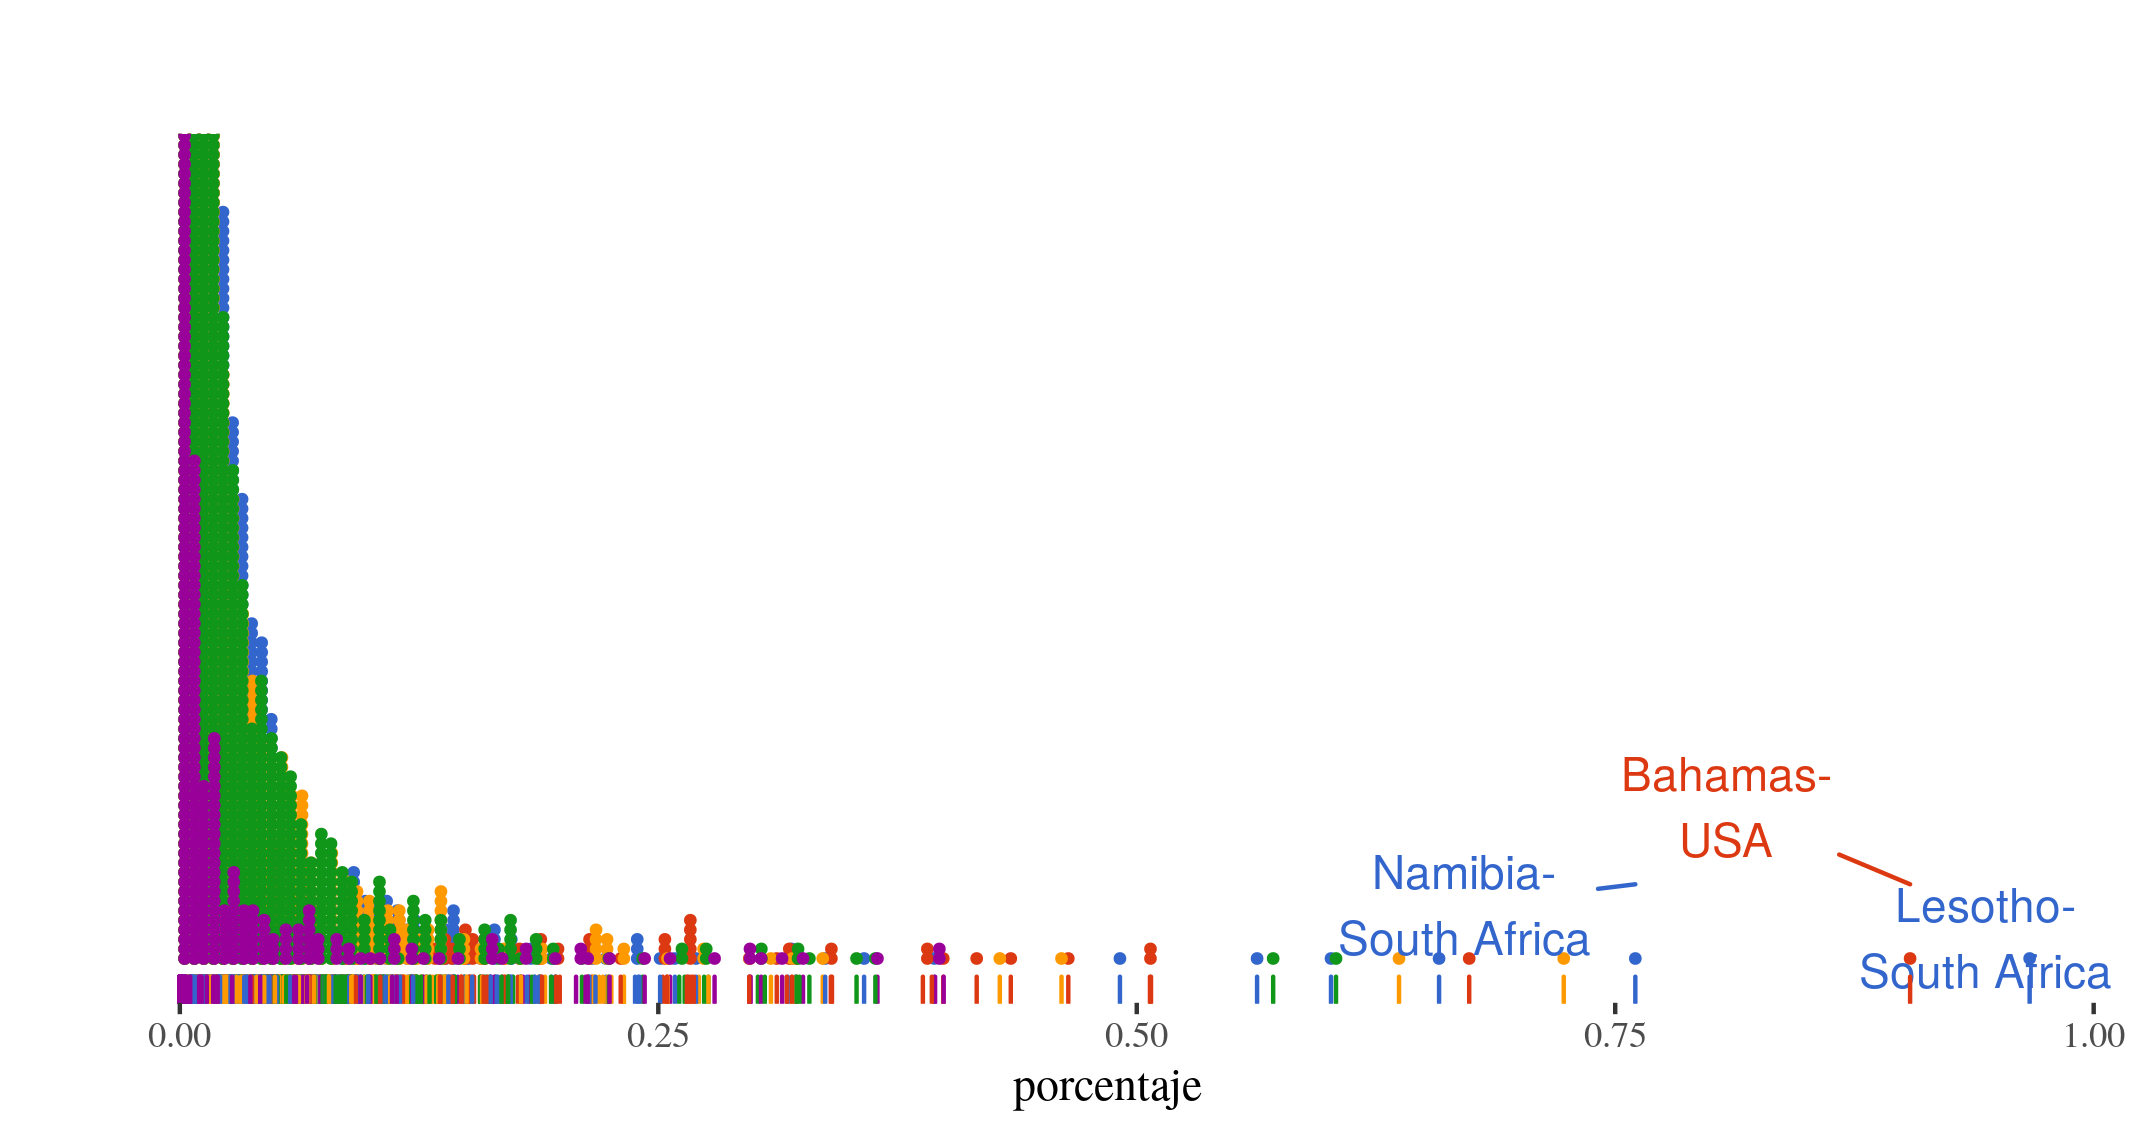
\includegraphics[scale=.5]{2011_freq_interacciones_3}
    \caption{}
    \label{fig:2011_freq_interacciones_3}
\end{figure}

Por su parte, en la imagen \ref{fig:2011_freq_interacciones_0} se puede apreciar una distribución similar en lo que respecta a los montos comerciados. Dado que esta expresado en términos absolutos, aquellas interacciones de mayor valor resultan de importancia para ambos polos de la relación. En particular, China aparece como un país con las relaciones comerciales de mayor volumen. A su vez, se observa que las relaciones comerciales de África no aparecen en el gráfico por estar truncado para los primeros bins, lo cual indica que los montos comerciados por dichos países, a pesar de representar una proporción muy grande en ciertos casos como se observó en el gráfico \ref{fig:2011_freq_interacciones_3}, son igualmente bajos respecto del resto del comercio mundial.


\begin{figure}[h]
    \centering
    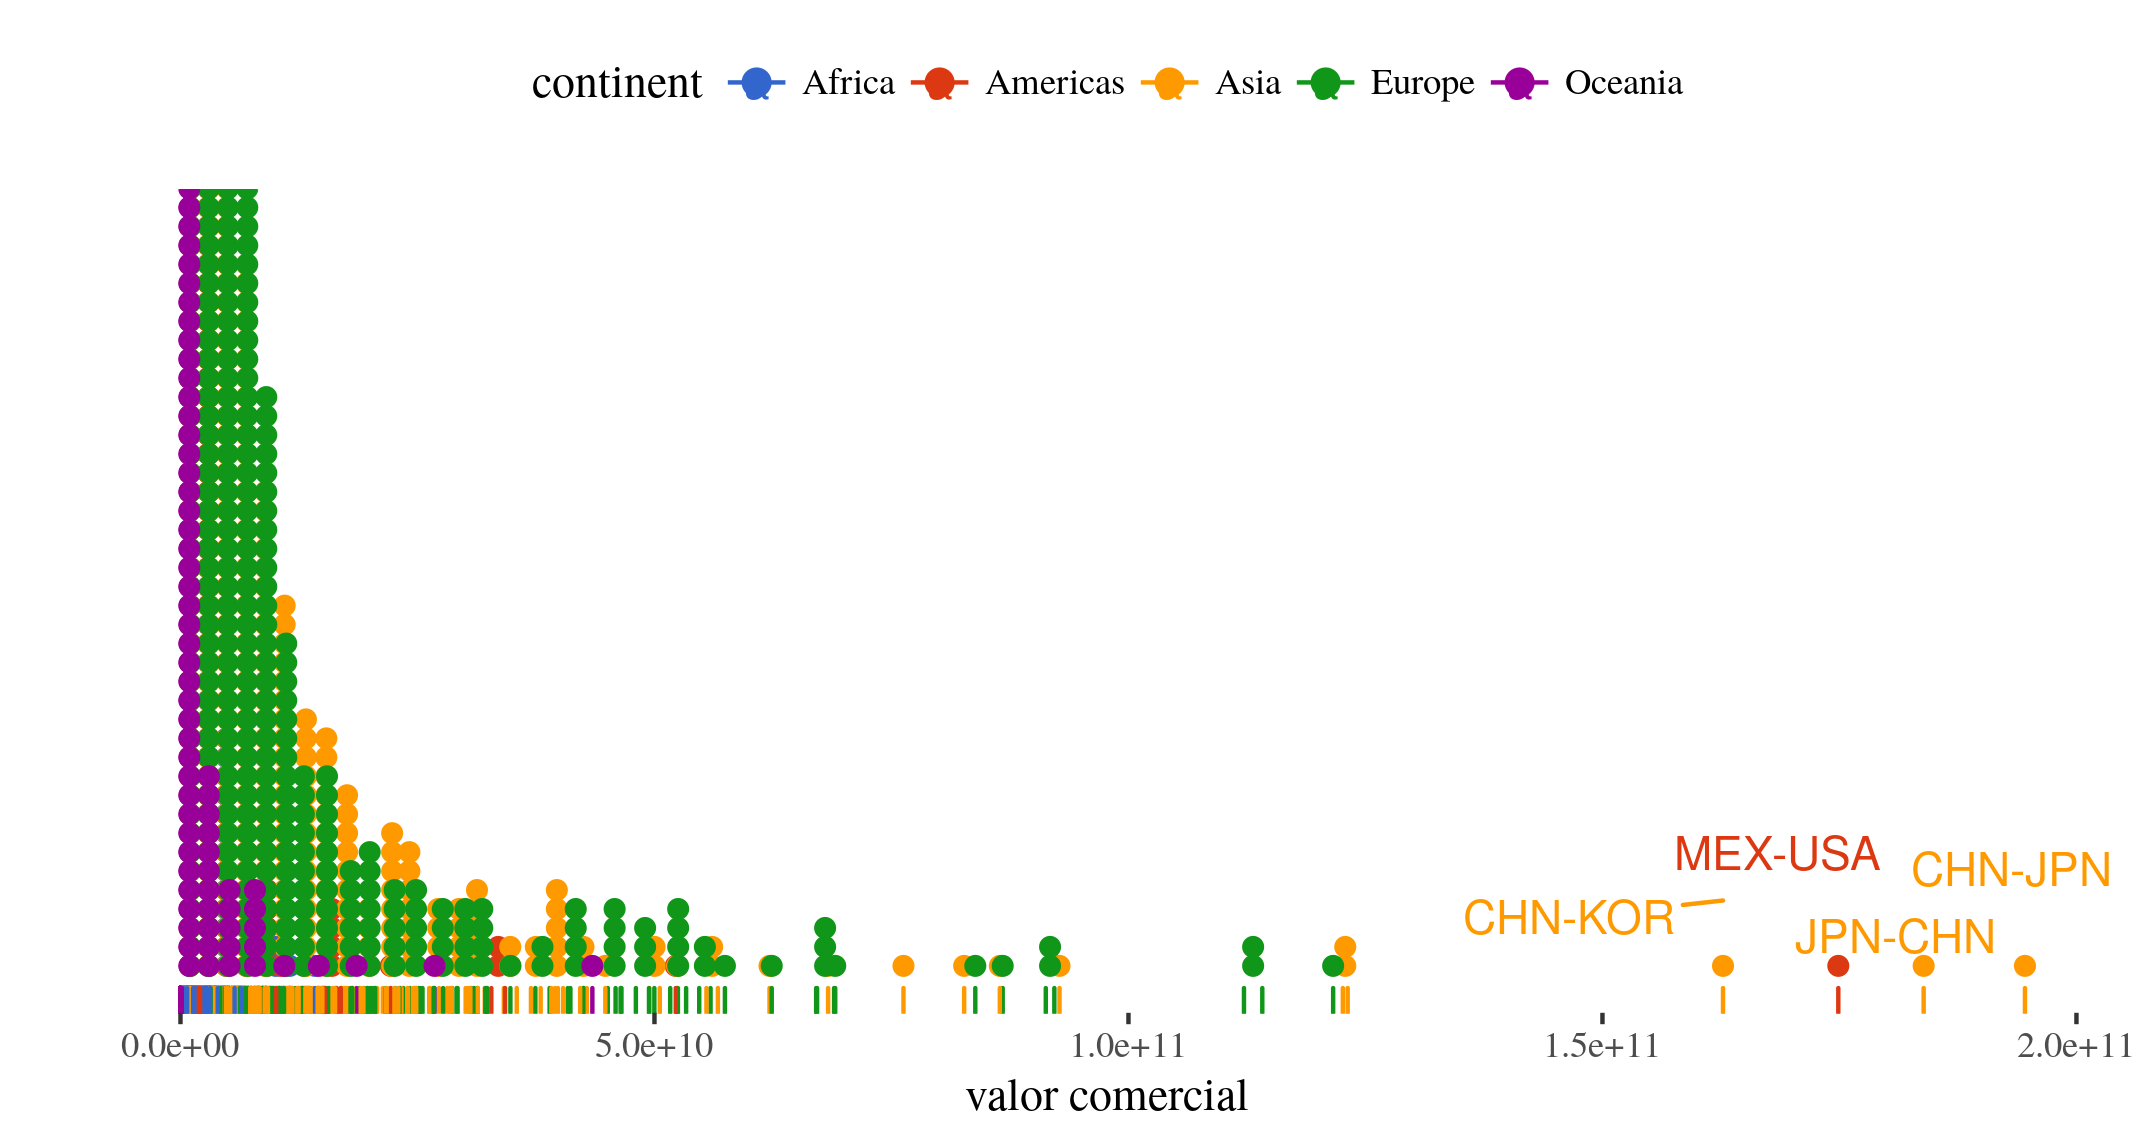
\includegraphics[scale=.5]{2011_freq_interacciones_0}
    \caption{}
    \label{fig:2011_freq_interacciones_0}
\end{figure}


\subsection{Determinación del punto de corte}

Para establecer un porcentaje de las importaciones como punto de corte para construir el grafo no ponderado se procedió construyendo grafos con un threshold entre 0 y 0.5, con incrementos de 0.01, para luego calcular distintas métricas que caracterizan al grafo, y buscar aquel punto en que se marque una inflección. En particular, se calculo si es un grafo conectado, el diámetro, la densidad, el número de aristas, la intermediación promedio y máxima, la cercanía promedio, el grado promedio, el autovalor promedio y el autovalor promedio ponderado por el valor comercial de la interacción, el coeficiente de clustering y la correlación de grado entre las aristas.

Los resultados arrojaron que el grafo resultante nunca es fuertemente conectado, aunque es débilmente conectado hasta un threshold de 10%. 
Como se observa en el gráfico \ref{fig:2011_autovalor_medio_x_threshold}, el autovalor medio de la red disminuye fuertemente al considerar un punto de corte del 1\%, y luego el descenso es más moderado. Lo mismo ocurre con el coeficiente de clustering, número de aristas y grado medio de la red. Por su parte, la intermediación promedio de la red tiene un máximo en el 1\%, para luego descender. Otras medidas, sin embargo, como la cercanía promedio, la intermediación máxima, el diámetro de la red o la correlación de grado, no muestran un comportamiento tan claro.

\begin{figure}[h]
    \centering
    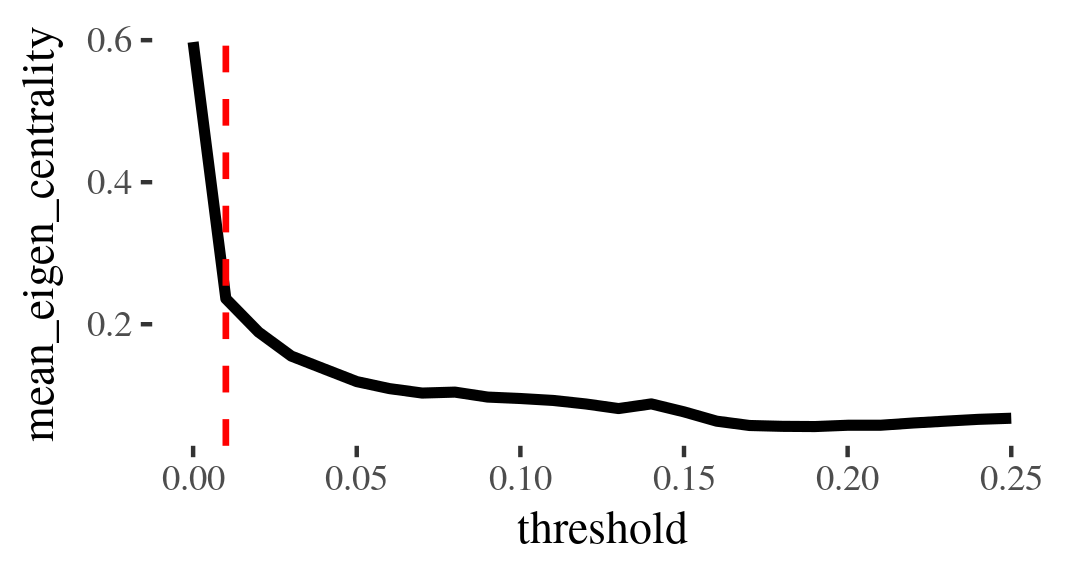
\includegraphics[scale=.5]{2011_autovalor_medio_x_threshold}
    \caption{}
    \label{fig:2011_autovalor_medio_x_threshold}
\end{figure}

Por ello, se decidió utilizar como referencia el 1\% para establecer el punto de corte, a la vez que se consideran otros puntos de corte alternativos para ciertos análisis particulares.

Se presentan a continuación los grafos para distintos puntos de corte que pueden resultar de interés.


\begin{figure}%
\centering
\begin{subfigure}{.3\linewidth}
\label{fig:grafo_2011-a}%
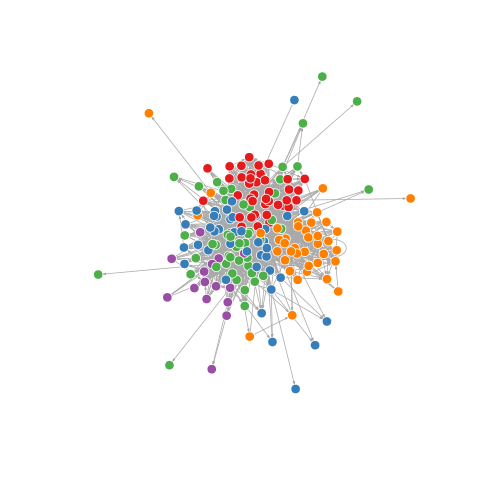
\includegraphics[width=\linewidth]{grafo_2011_1_pcnt}%
\end{subfigure}%
\begin{subfigure}{.3\linewidth}
\label{fig:grafo_2011-c}%
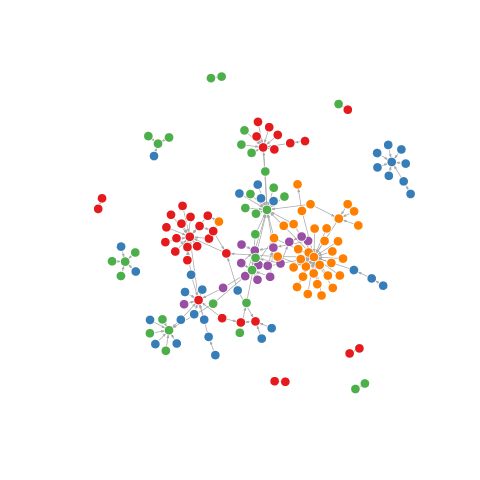
\includegraphics[width=\linewidth]{grafo_2011_15_pcnt}%
\end{subfigure}%
\begin{subfigure}{.3\linewidth}
\label{fig:grafo_2011-b}%
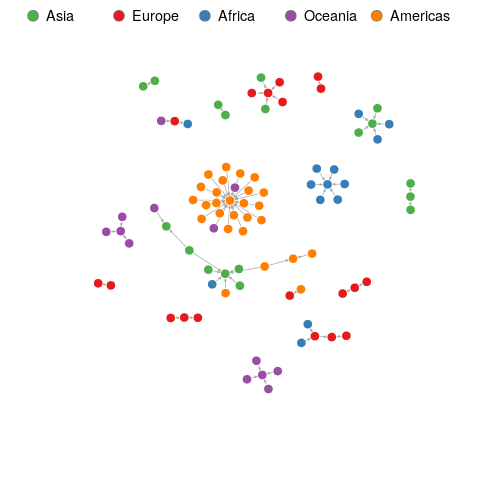
\includegraphics[width=\linewidth]{grafo_2011_25_pcnt}%
\end{subfigure}
\caption[]{}%
\label{fig:grafo_2011}%
\end{figure}



En los grafos representados se puede observar como hasta un punto de corte del 10\% la red se mantiene unida, aunque disminuye la cantidad de nodos. A partir de este punto, la red deja de estar débilmente conectada y, a la vez que sigue disminuyendo la cantidad de nodos, se observa mejor la importancia de ciertos nodos de alto grado. En particular, uno del continente americano (Estados Unidos) y otro del continente africano (Sudáfrica).


\subsection{Correlación entre la representación de las exportaciones y las importaciones}

Por su parte, dada la potencial diferencia en el análisis si se tiene en cuenta las exportaciones y las importaciones, se incorporó esta disyuntiva como una nueva dimensión de análisis. Para ello, se considero el grado total de cada nodo, para un grupo de puntos de corte, para el grafo que surge de considerar las exportaciones y las importaciones. En el gráfico \ref{fig:corr} se pueden observar los resultados.



\begin{figure}%
    \begin{subfigure}{\linewidth}
        \centering
        \label{fig:corr-a}%
        \caption{}
        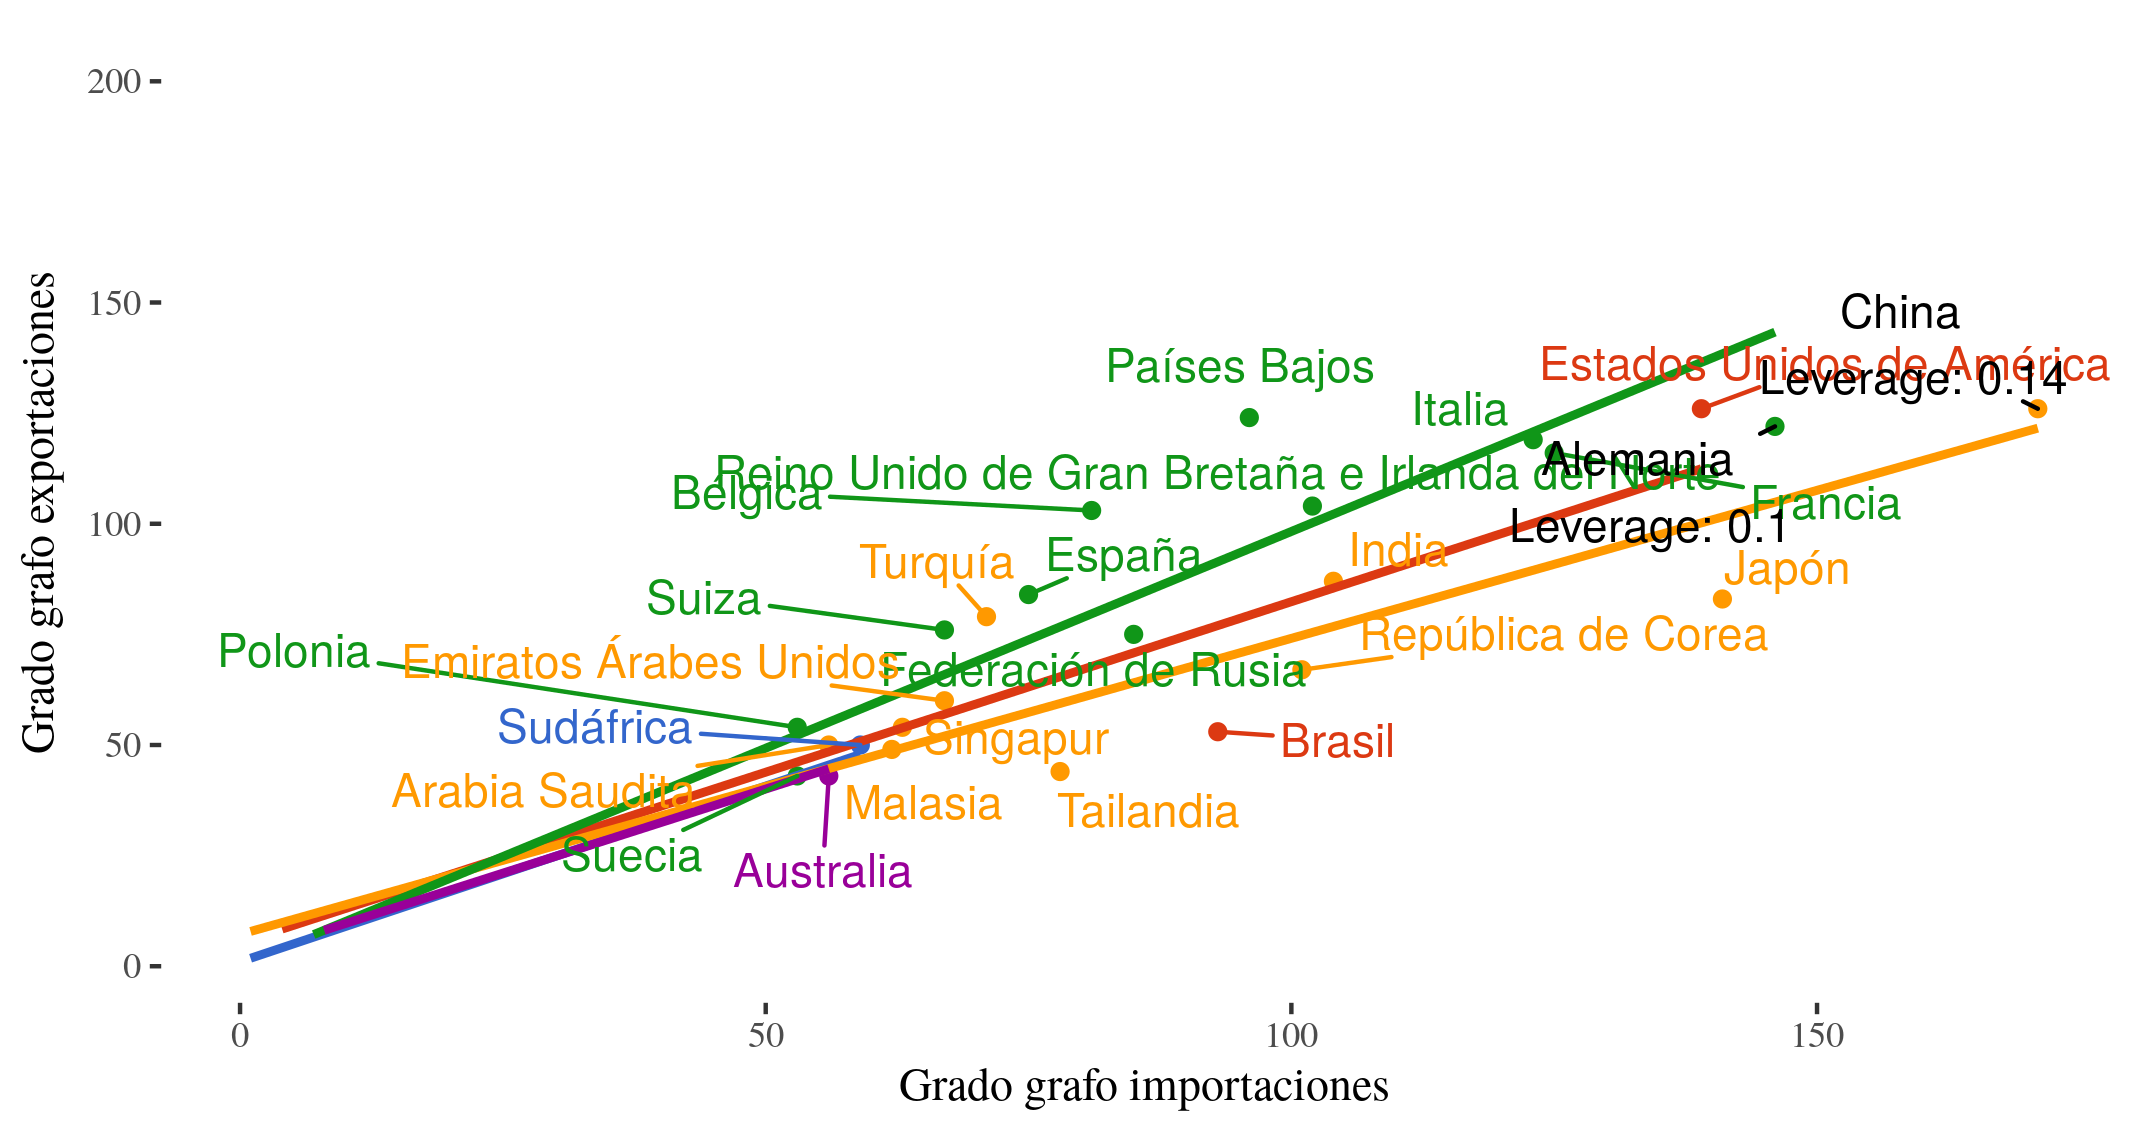
\includegraphics[width=\linewidth]{corr_grados_2011_1_pcnt}
    \end{subfigure}%
    
    \begin{subfigure}{\linewidth}
        \centering
        \label{fig:corr-b}%
        \caption{}
        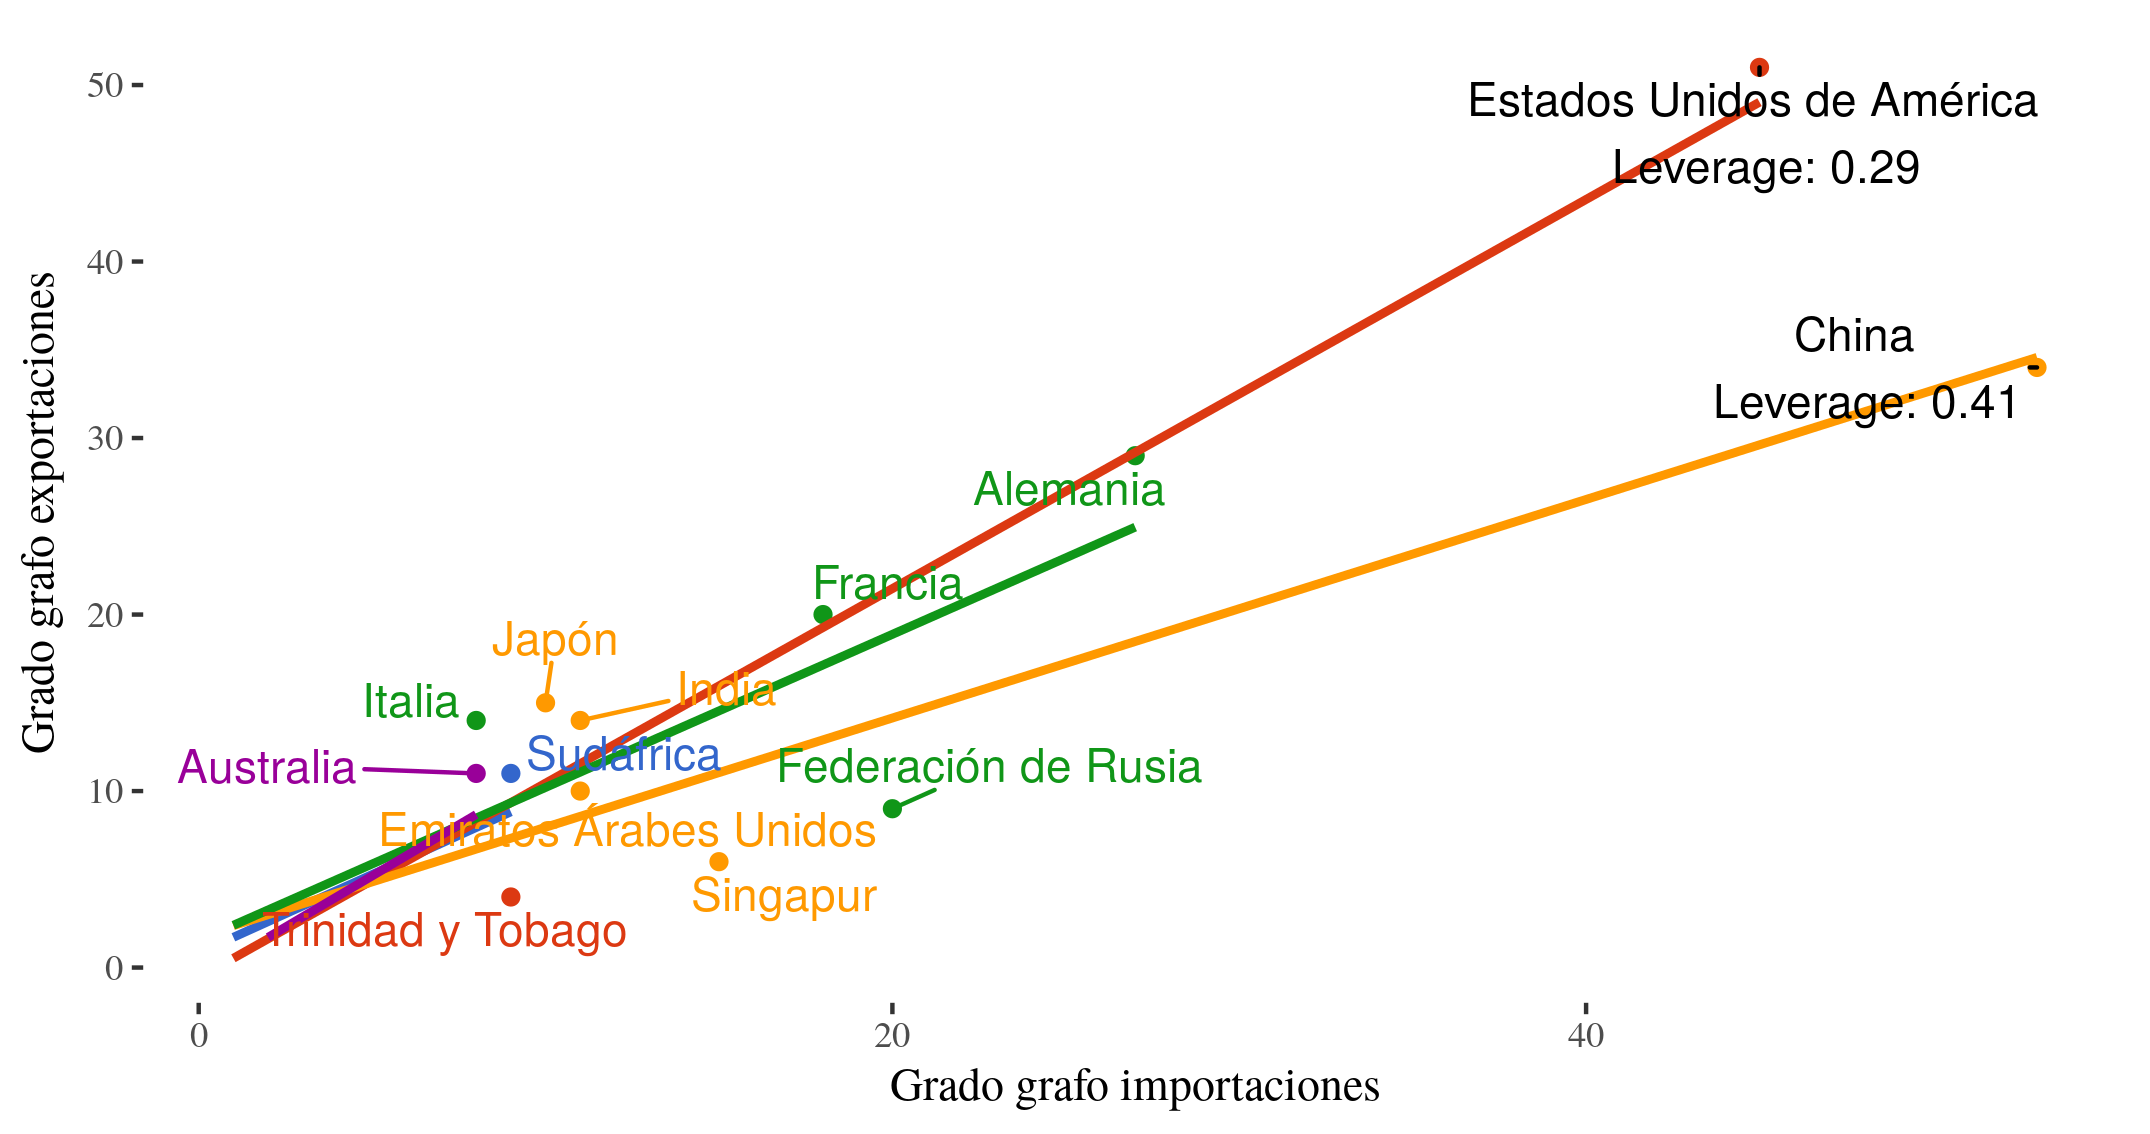
\includegraphics[width=\linewidth]{corr_grados_2011_10_pcnt}
    \end{subfigure}

    \begin{subfigure}{\linewidth}
        \centering
        \label{fig:corr-c}%
        \caption{}
        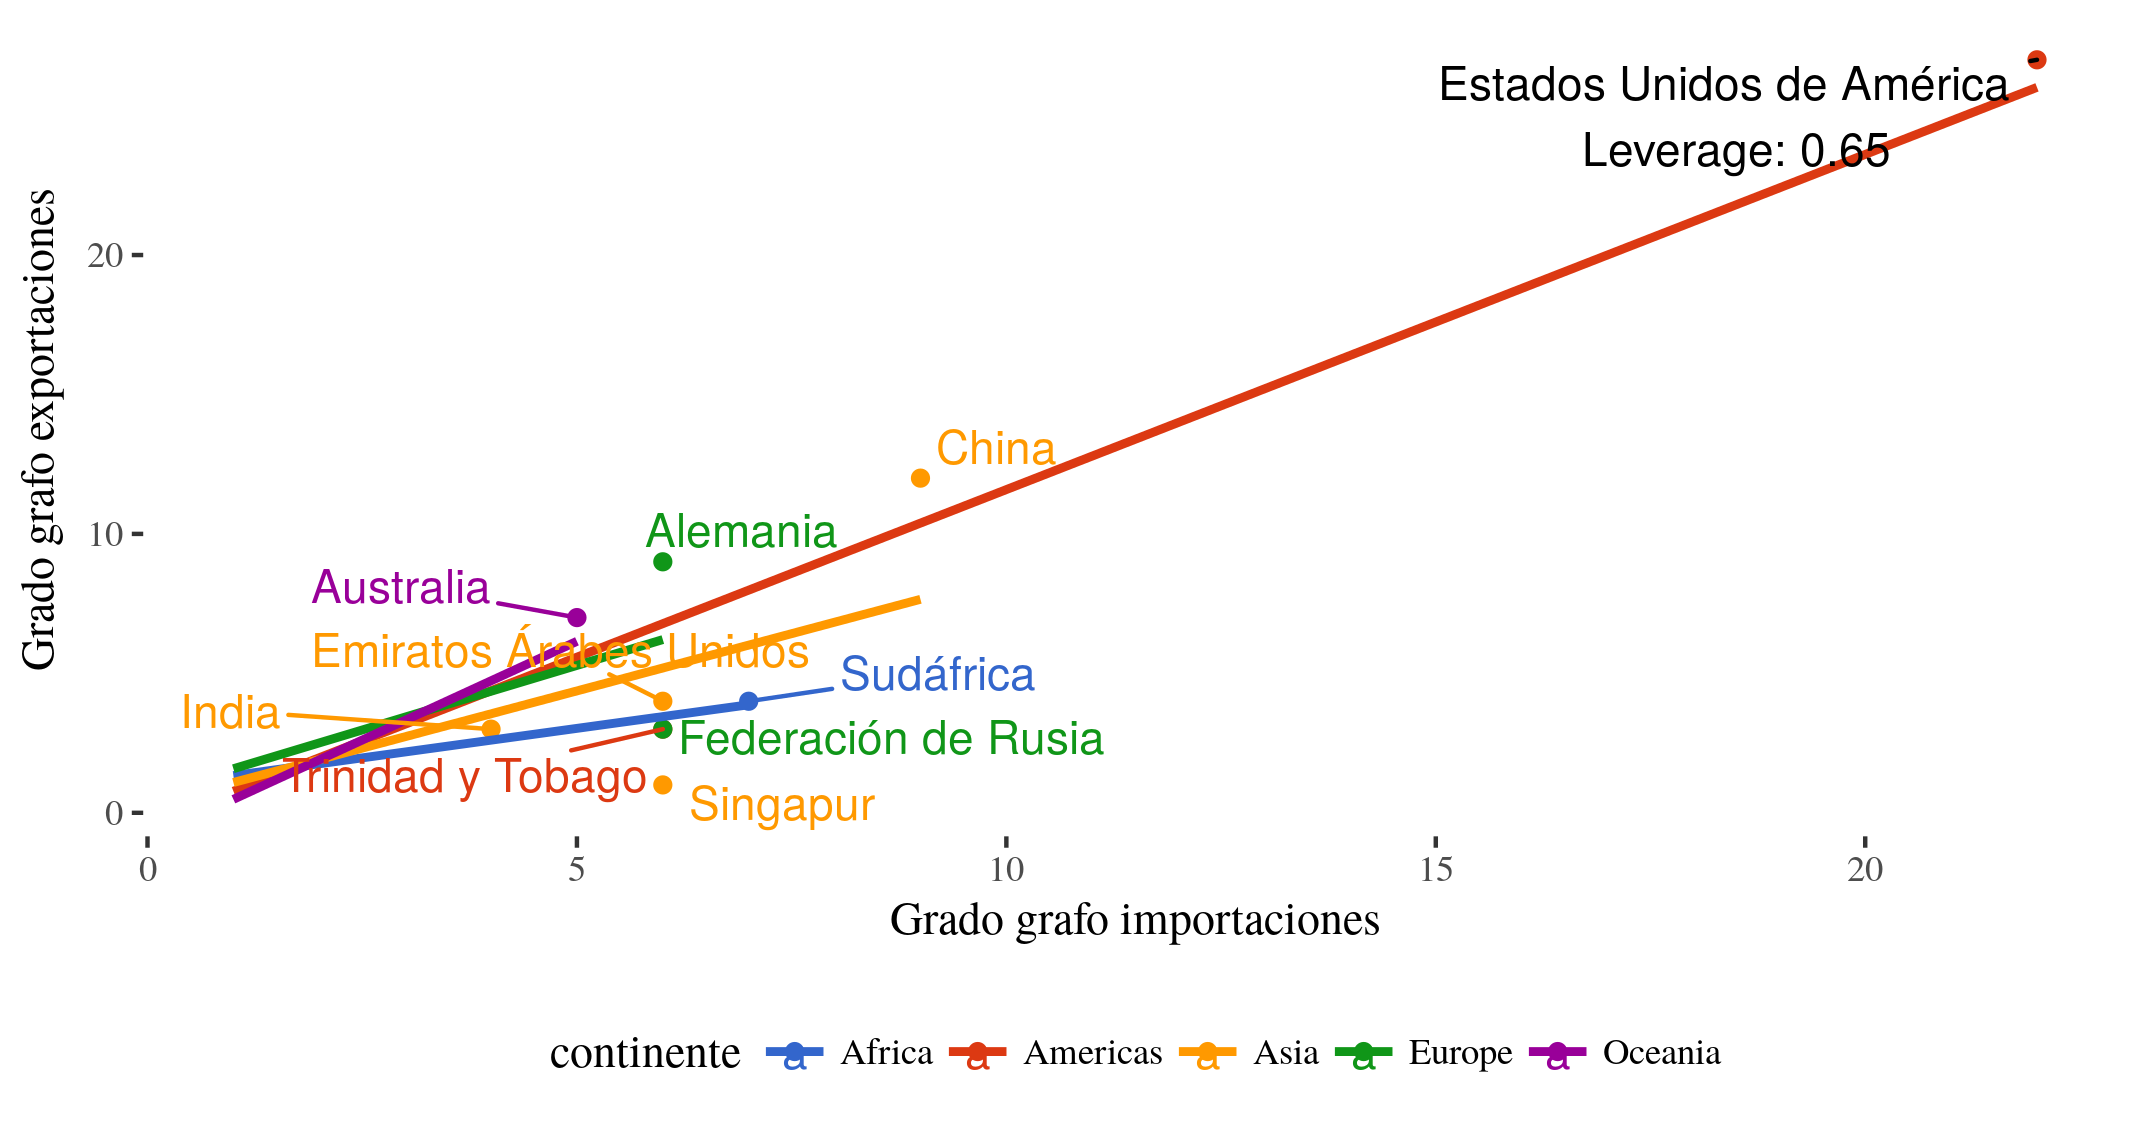
\includegraphics[width=\linewidth]{corr_grados_2011_20_pcnt}%
    \end{subfigure}
    \caption[]{}%
    \label{fig:corr}%
\end{figure}

La correlación entre los grafos resultantes oscila entre el 0.84 y 0.95 si se consideran puntos de corte de entre el 1\% y el 25\%, por lo que se puede considerar que al observar las importaciones no se pierde demasiada información. 
Sin embargo, surgen algunas diferencias interesantes. La regresión lineal para cada continente, muestra el diferente rol de éstos en el mercado mundial, donde Asia se presenta en el rol de productor de mercancías, mientras que Europa lo hace como un gran consumidor del mercado mundial. El caso americano tiene por un lado el rol preponderante de Estados Unidos, con un comportamiento similar al de Europa (con independencia del threshold del 0.25), mientras que el resto del continente, junto con Oceanía y África, juegan un rol secundario. En el caso europeo, se observa como Rusia tiene un comportamiento más acorde al continente asiático, mientras que en este último se destacan en particular China y Singapur como grandes productores. 
Sin embargo, el rol de cada país varía también respecto al threshold considerado. En el caso de Japón, en puntos de corte bajos, donde hay relaciones comerciales de importancia moderada para los países, se presenta jugando un rol de productor más que de consumidor, incluso más que la media asiática. A medida que se aumenta el punto de corte, y por lo tanto se consideran exclusivamente relaciones de carácter más dependiente, Japón se presenta como un país consumidor, incluso más que los países europeos. Esta transición estaría indicando que Japón, productor de productos industriales y tecnológicos, provee a muchos países del mundo de este tipo de mercancías, aunque éstos no dependen en su consumo de Japón, mientras que como consumidor de materias primas, este país establece relaciones comerciales con países que sí dependen de Japón para poder colocar sus mercancías. En el caso de China se puede observar algo similar, aunque de forma más moderada. Más interesante aún, a medida que se consideran relaciones de tipo más dependiente, aparece como destacado el rol de Estados Unidos, relegando a los países europeos y asiáticos. Por su parte, también surge Sudáfrica como un jugador importante del mercado mundial, cuando se consideran este tipo de relaciones de mayor dependencia. Esto implica que estos dos países tienen una forma de interacción en el mercado mundial marcadamente diferente a la de los países europeos y asiáticos.
Por último, en el gráfico \ref{fig:corr} se puede observar el leverage de las ĺos países con mayor apalancamiento para la regresión del grado de las exportaciones respecto del de las importaciones, sin diferenciar por continente. Cuando se considera un punto de corte del 1\%, China tiene el mayor leverage, con un número bastatne mayor que Estados Unidos, aunque el valor es relativamente bajo. Sin embargo, a medida que se consideran puntos de corte más altos, Estados Unidos se constituye como el país con mayor apalancamiento en la regresión, a la vez que el valor aumenta fuertemente. 
A continuación se presenta el top 5 de países de mayor centralidad de grado para el 2011, en el grafo de importaciones y en el de exportaciones.

\begin{table}[]
\centering
\caption{}
\label{Table: Tabla1}
\begin{tabular}{llclc}
 & \multicolumn{2}{l}{Grafo Importaciones} &  \multicolumn{2}{l}{Grafo Importaciones} \\
 Orden &           País &          G \degree entrada &           País & G \degree entrada          \\
  1\degree &           CHN &          155 &           USA & 126         \\
  2\degree &           USA &          149 &           NLD & 106         \\
  3\degree &           DEU &          129 &           GBR & 104         \\
  4\degree &           JPN &          124 &           CHN & 103         \\
  5\degree &           FRA &          112 &           DEU & 101        
\end{tabular}
\end{table}

La tabla \ref{Table: Tabla1} muestra como tanto China, como Estados Unidos y Alemania son nodos de una centralidad importante, tanto como consumidores como en su rol de productores. Sin embargo, China se destaca más en este último sentido que en el primero. Por su parte, Estados  Unidos marca una importante como consumidor respecto de los Países Bajos, aunque no conserva tal hegemonía como productor global. 

\section{Análisis 1997-2011}

Lo que resta del análisis se considerará exclusivamente el punto de corte del 1\%, incorporando la dimensión temporal. Para esto, se considerará en primer lugar el movimiento de algunas medidas de resumen a lo largo del tiempo, para luego analizar la distribución de algunas medidas de centralidad y el cambio en el rol de los nodos centrales en durante el período.


\subsection{Medidas de resumen de la red}

A continuación se presentan los valores de algunas medidas de resumen entre el período de 1997 y 2011, considerando un punto de corte del 1\% para las exportaciones. 

\begin{figure}%
\centering
\begin{subfigure}{.45\linewidth}
\label{fig:caracteristicas_yr-a}%
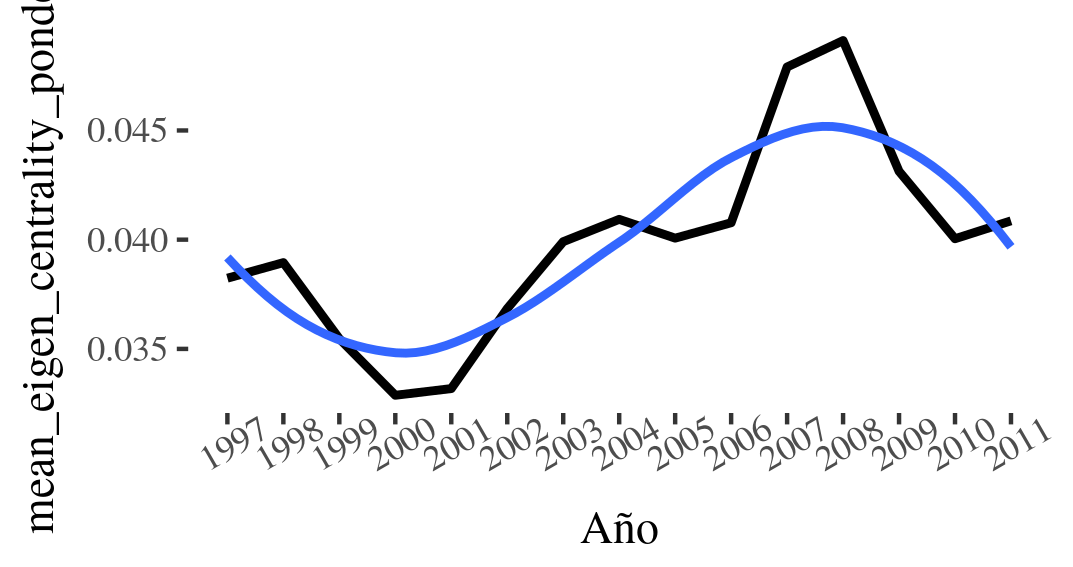
\includegraphics[width=\linewidth]{mean_eigen_centrality_ponderado_x_yr}%
\end{subfigure}%
\begin{subfigure}{.45\linewidth}
\label{fig:caracteristicas_yr-b}%
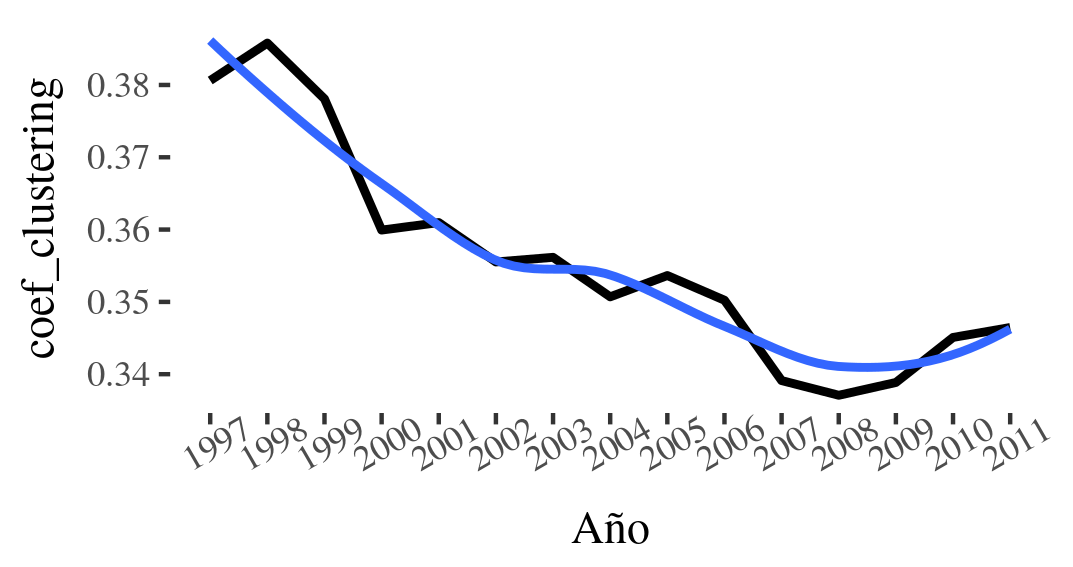
\includegraphics[width=\linewidth]{coef_clustering_x_yr}%
\end{subfigure}%
\caption[]{}%
\label{fig:caracteristicas_yr}%
\end{figure}

Como se puede observar, las características topológicas del grafo varían fuertemente en el período 2007-2009, durante la gran recesión económica, que se caracterizó por un aumento en el proteccionismo económico de ciertos países centrales, reflejado en el “Buy American”\footnote{http://edition.cnn.com/2009/POLITICS/02/05/senate.buy.american/index.html} o “Buy China” \footnote{https://economix.blogs.nytimes.com/2009/06/29/buy-china/}. 
La caída de la correlación de grado en el año 2007 implica una transición circunstancial hacia una economía menos selectiva. Es decir, un comercio internacional donde aumentan las relaciones de nodos de mayor grado con nodos de menor grado, respecto de las relaciones entre nodos de similar magnitud. 
Por su parte, el coeficiente de clustering tiene una tendencia decreciente hasta 2008, para luego comenzar a crecer nuevamente. Esto se puede interpretar como una de-segmentación del comercio internacional hasta la crisis, con al cual comienza un proceso de re-segmentación. 
El autovalor promedio de la red ponderada tiene un comportamiento particularmente extraño, con un mínimo durante el período de la crisis de 2001, y un máximo en la crisis de 2008, 2009.
Dados estos resultados, se considera que sería prematuro asociar ciertas características topológicas de la red con la eminencia o emergencia de una crisis internacional, aunque sí pareciera que de conjunto existen importantes cambios. Para poder determinar con certeza las relaciones planteadas, sería necesario contar con un mayor rango temporal, donde se puedan observar varias crisis comerciales.

\subcaption{Distribución de los nodos}

a continuación se presenta la distribución de los nodos según ciertas medidas de centralidad a lo largo de los años, destacando aquellos países con mayores valores de centralidad. 

\begin{figure}%
    \begin{subfigure}{.5\linewidth}
        \centering
        \label{fig:corr-a}%
        \caption{}
        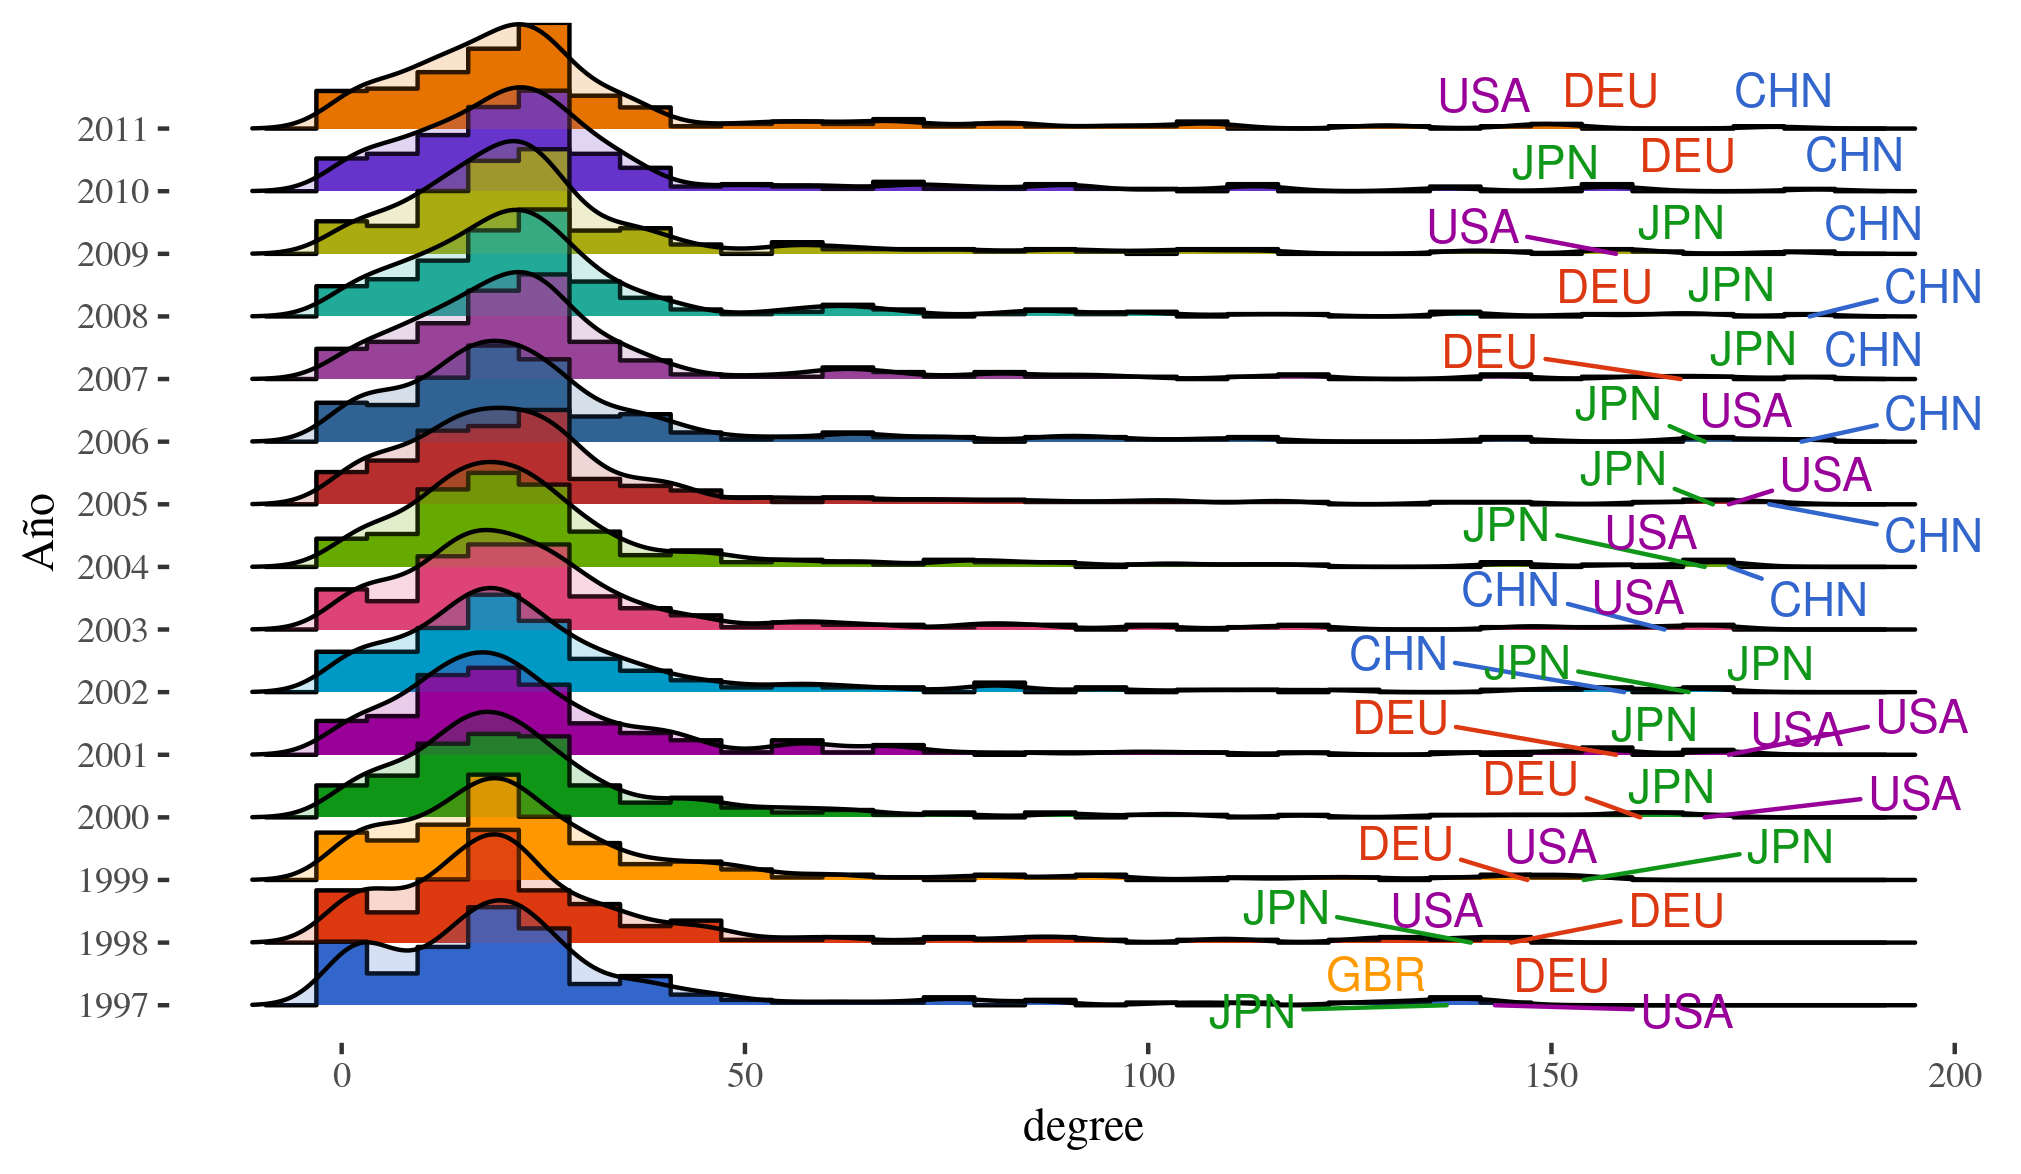
\includegraphics[width=\linewidth]{impo_densidad_degree_x_yr}
    \end{subfigure}%
    
    \begin{subfigure}{.5\linewidth}
        \centering
        \label{fig:corr-b}%
        \caption{}
        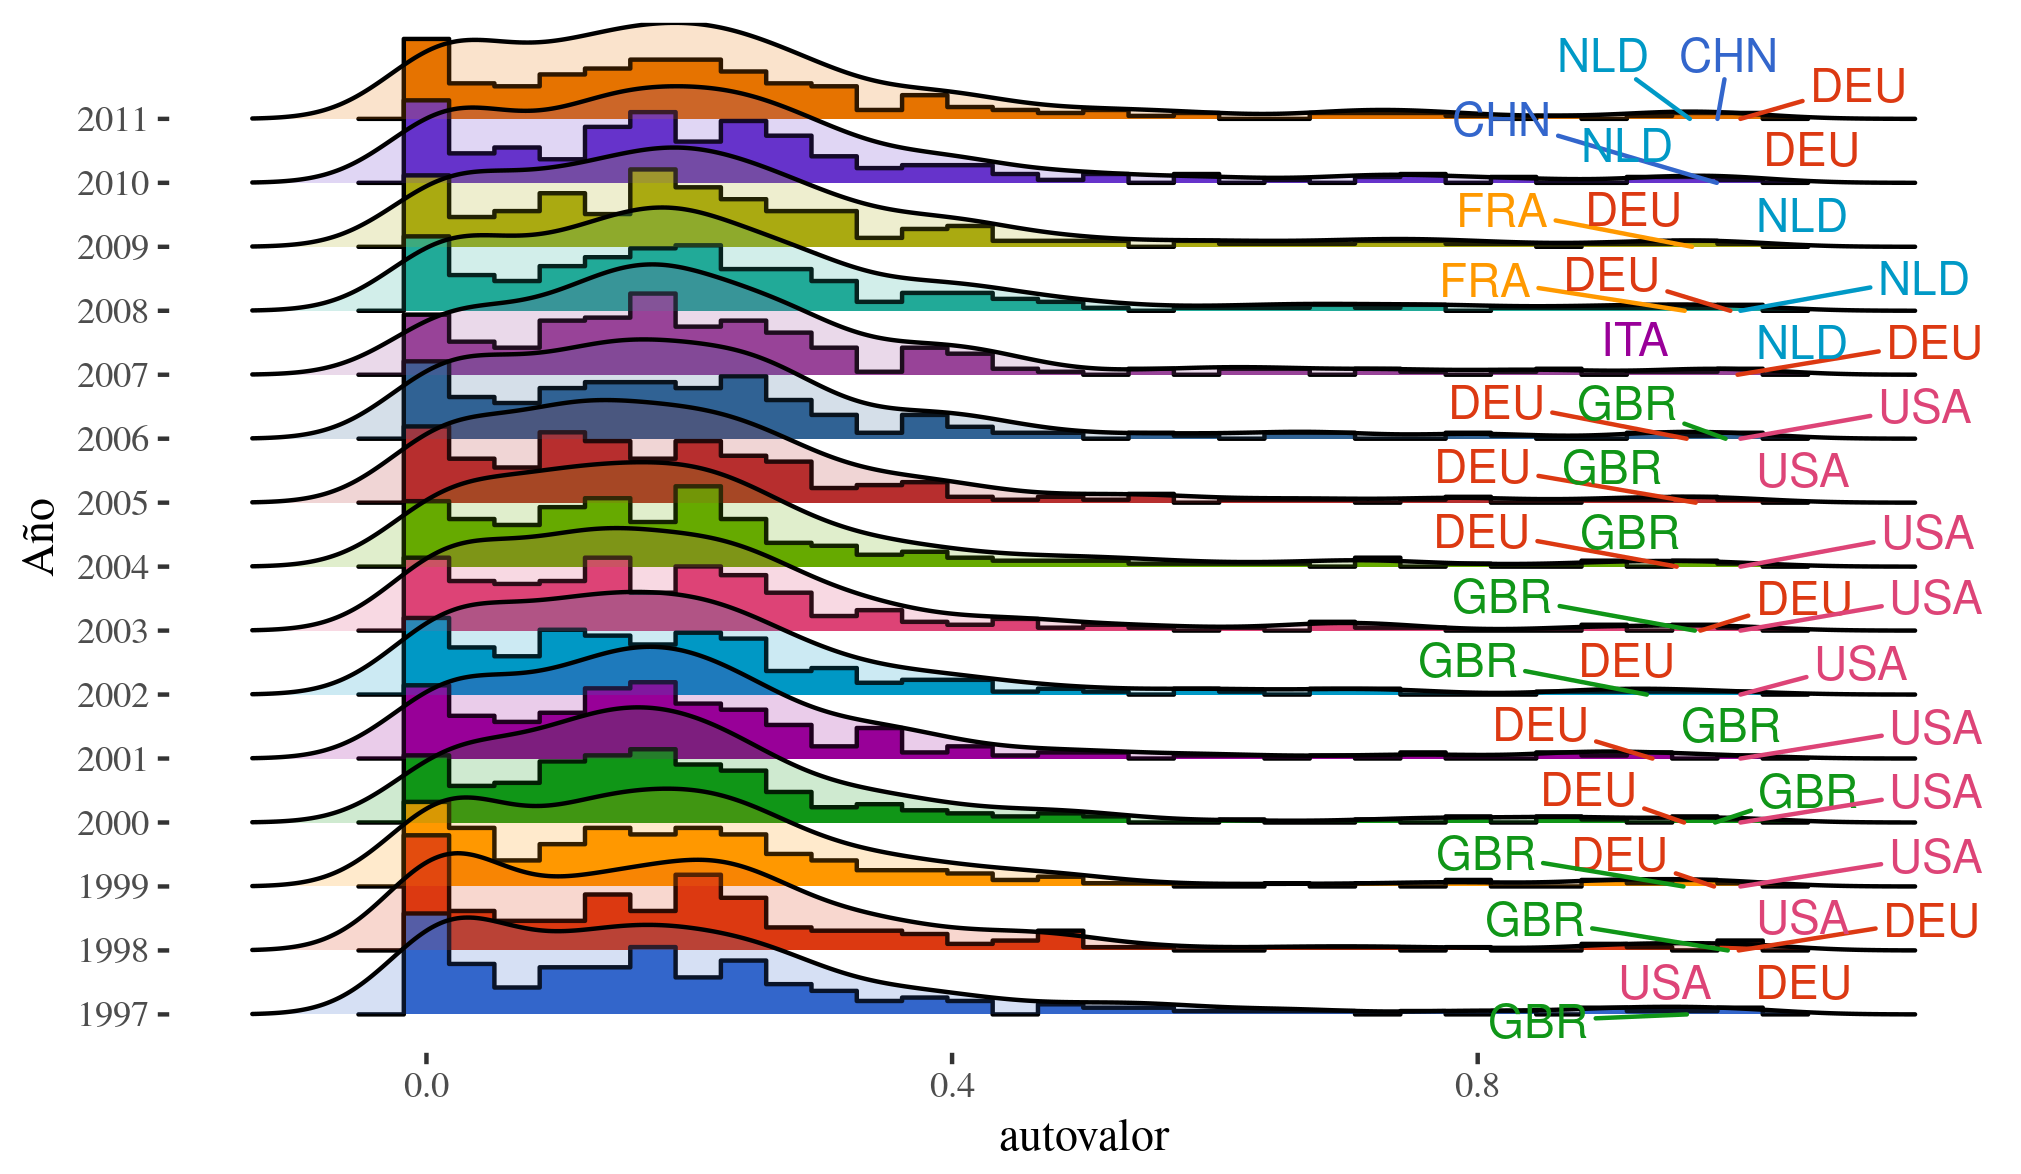
\includegraphics[width=\linewidth]{expo_densidad_autovalor_x_yr}
    \end{subfigure}

    \begin{subfigure}{.5\linewidth}
        \centering
        \label{fig:corr-c}%
        \caption{}
        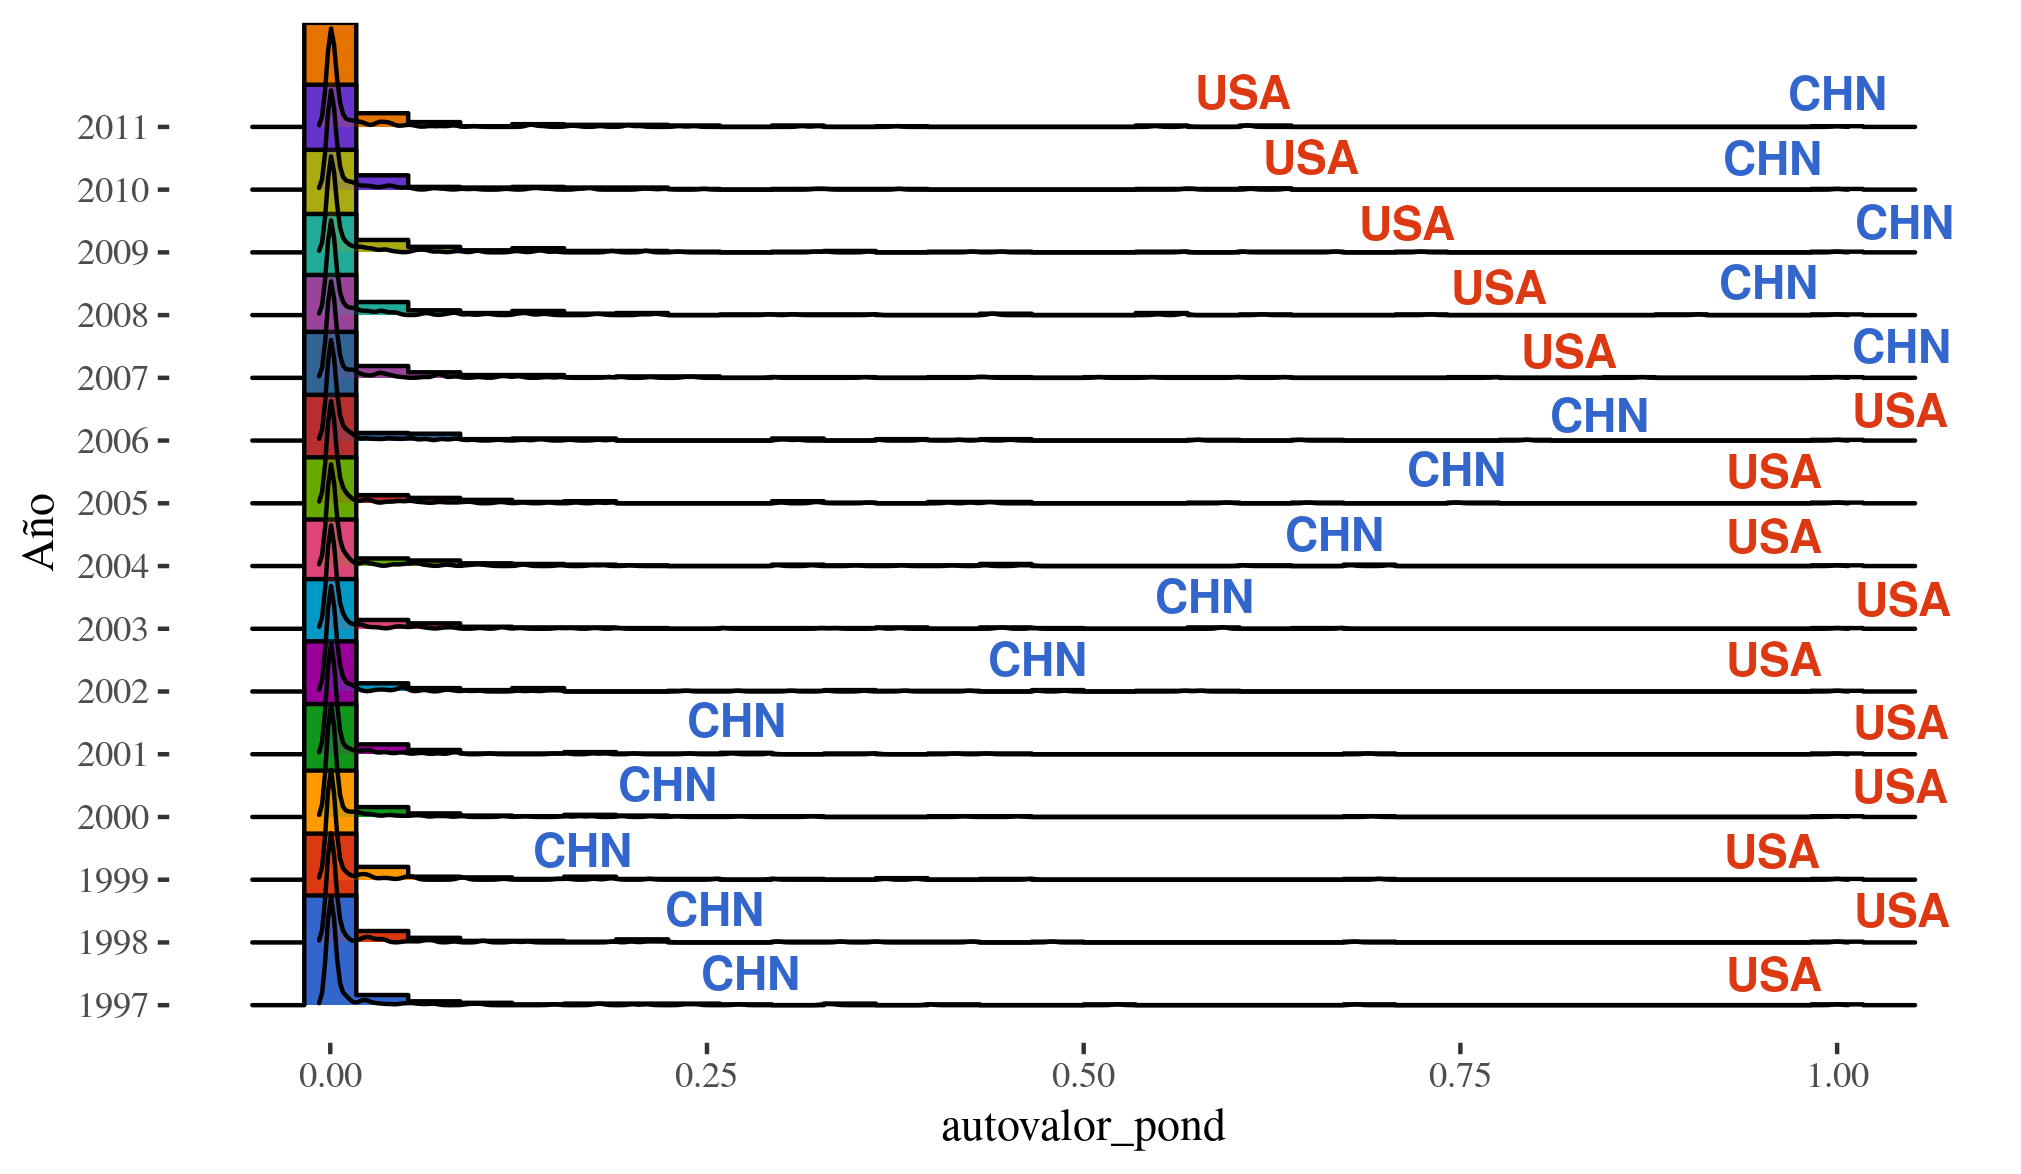
\includegraphics[width=\linewidth]{expo_densidad_USAvsCHN_autovalor_pond_x_yr}%
    \end{subfigure}
    
    \begin{subfigure}{.5\linewidth}
        \centering
        \label{fig:corr-c}%
        \caption{}
        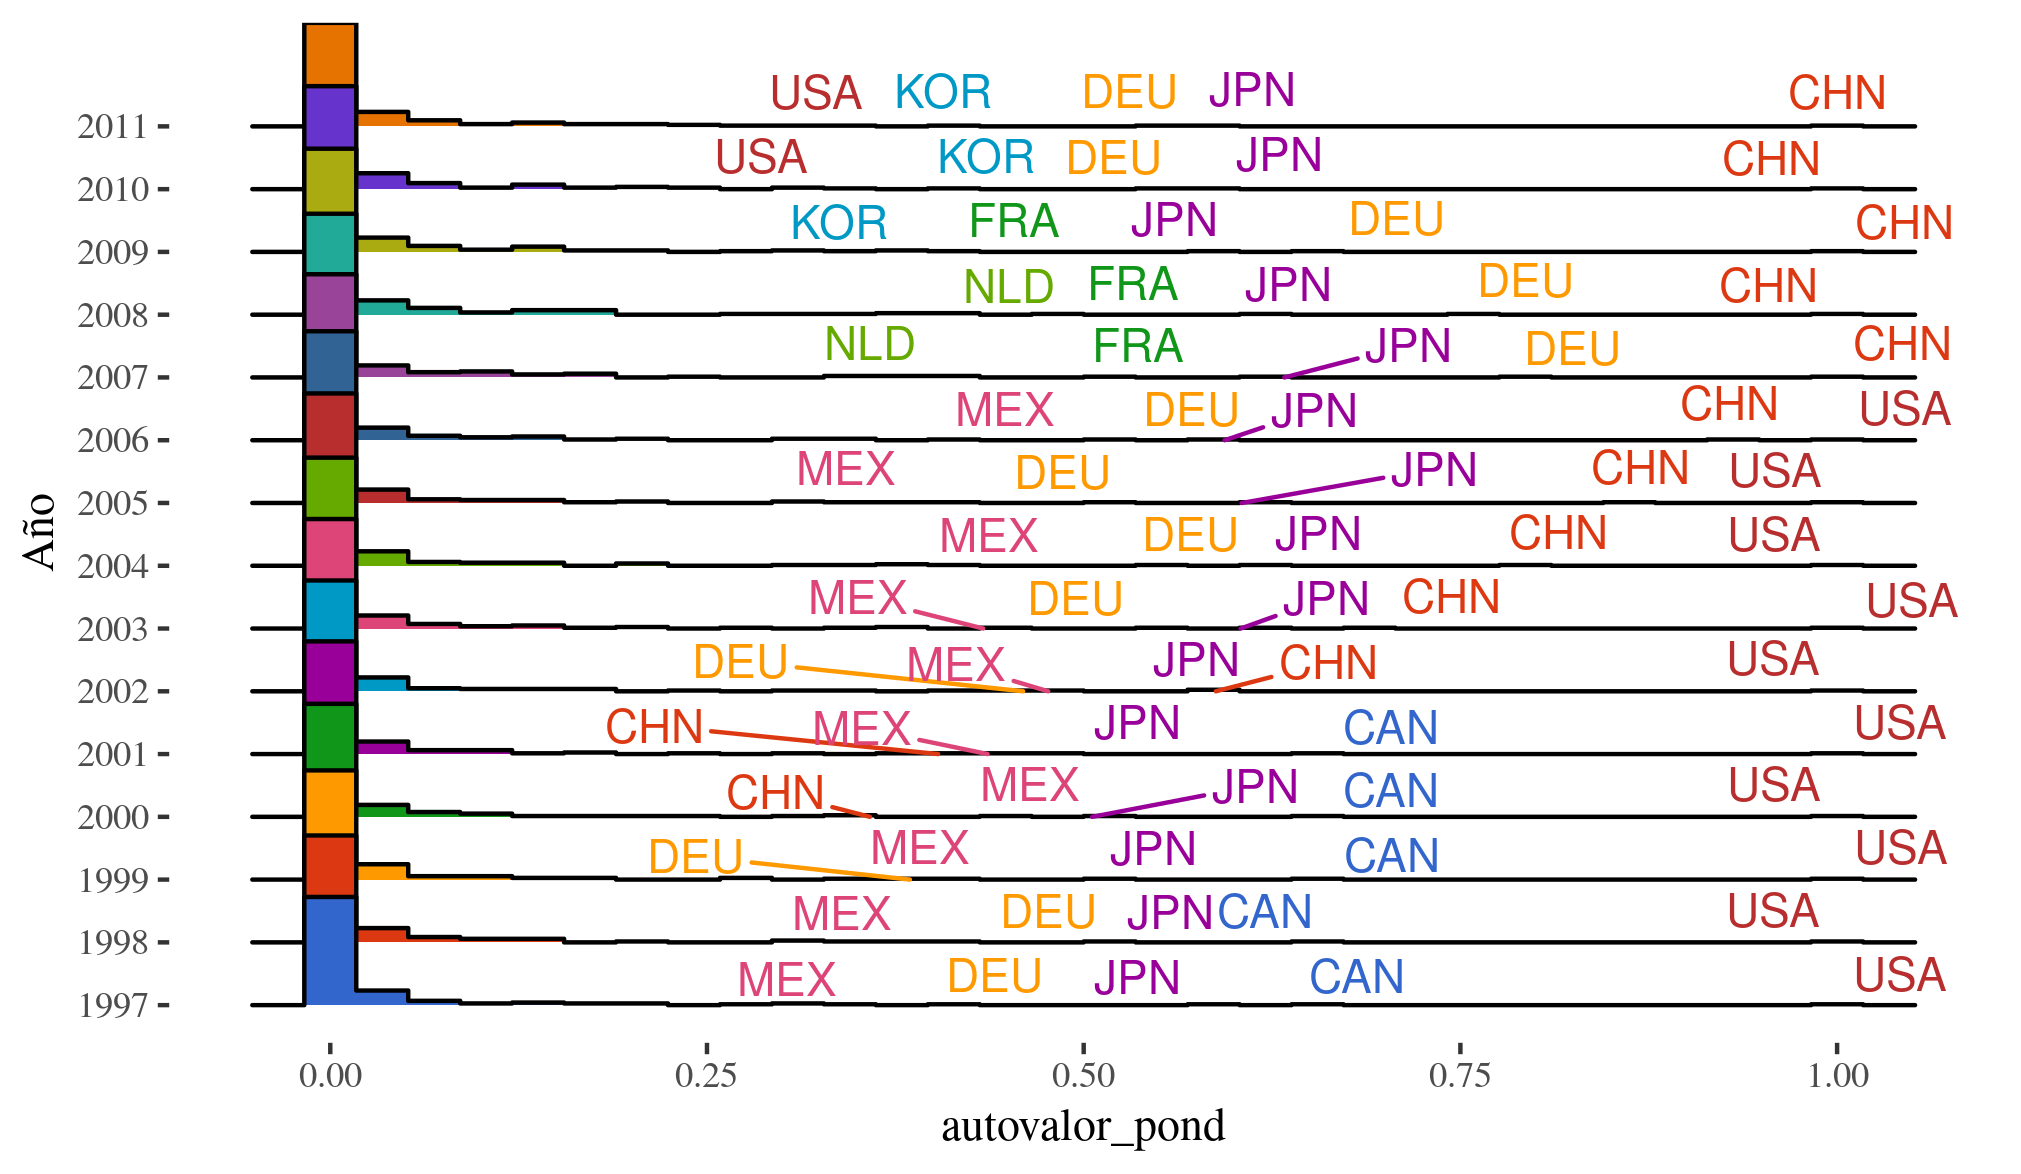
\includegraphics[width=\linewidth]{impo_densidad_autovalor_pond_x_yr}%
    \end{subfigure}

\caption[]{}%
\label{fig:distribuciones}%
\end{figure}

En primer lugar, lo que se observa en el gráfico \ref{fig:distribuciones} es que la distribución de los nodos de acuerdo a las distintas medidas de centralidad no varía sustancialmente de año en año, ni en su rol como consumidores globales, ni en su rol como productores globales. Por su parte en la distribución de grado de los nodos del grafo de importaciones, se puede observar como los tres países de mayor grado tienden a alejarse del centro de masa de la distribución.  Este podio se disputa entre Alemania, Japón, Estados Unidos y, a partir del 2002, China, quien a su vez tiende a alejarse de éstos posteriormente. Por su parte, en el rol de consumidor global, se observa como, mientras hasta 2007 Estados Unidos y Gran Bretaña ocupan los lugares principales en la centralidad de autovalor, a partir de este año comienza a tener un rol más destacado Francia y los países bajos, y luego China. 
Por su parte, es de resaltar el aumento en la centralidad de China para el comercio internacional, tanto como productor como consumidor. En particular, este país desplaza a Estados Unidos de ser el nodo de mayor centralidad en muchas medidas. Por ejemplo, para el caso del autovalor ponderador por el valor del intercambio, Estados Unidos ocupa el primer lugar hasta el año 2006, para luego ser reemplazado por China, un país que diez años antes tenía un valor de centralidad cuatro veces menor al de Estados Unidos. En ese mismo año China también pasa a ocupar el primer lugar en dicha métrica para el grafo de las importaciones. La medida de centralidad del autovalor es particularmente relevante, sobretodo todo ponderada por el valor de las transacciones, porque considera no sólo la importancia del nodo, sino también la importancia de aquellos nodos con que se relaciona. En este sentido, se destaca el rol de México, Japón, Canadá, junto con China y Estados Unidos como grandes productores mundiales, a la vez que aparece, sobre los últimos años, Corea como una nueva potencia en este aspecto.  

\section{Búsqueda de comunidades}

Por último, se realizó un análisis de búsqueda de comunidades. Para ello, se utilizó el algoritmo de Louvain, que arrojó una modularidad de 0.27, que comparada con la modularidad de mil grafos de igual tamaño y una membresía asignada de forma aleatoria, resulta siempre mayor, indicando que los clusters encontrado por el algoritmo no surgen del azar.
En el gráfico \ref{fig:comunidades} se pueden observar los resultados de las comunidades encontradas, destacadas por forma y tamaño de los nodos, mientras que se utiliza el color del nodo para distinguir su continente de procedencia. 

\begin{figure}[h]
    \centering
    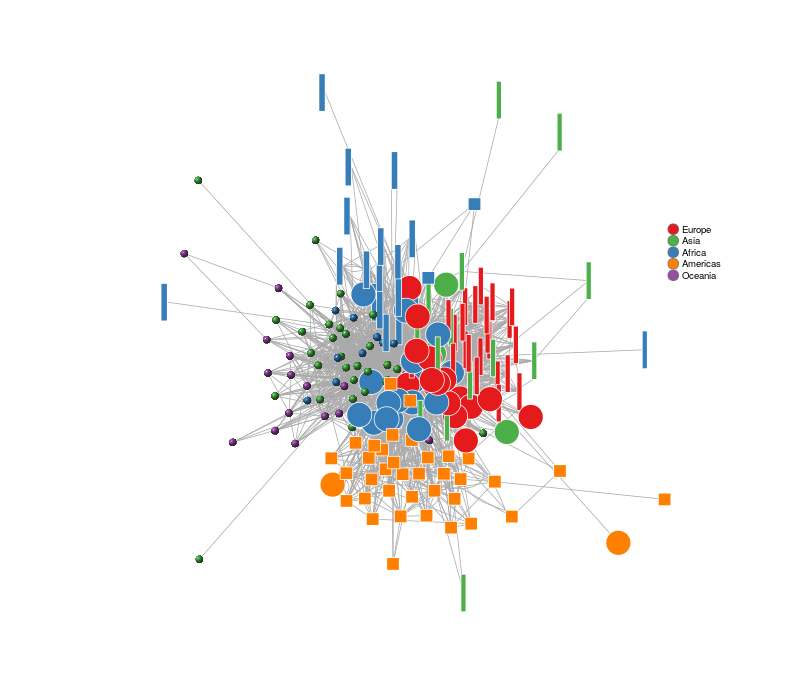
\includegraphics[scale=.5]{grafo_2011_comunidades}
    \caption{}
    \label{fig:comunidades}
\end{figure}


De aquí se destaca en primer lugar la correspondencia del continente americano con uno de los clusters encontrados por el algoritmo. Por su parte, existe un cluster que combina los países del continente Asiático con los de Oceanía, mientras que África y Europa quedan distribuidas en partes iguales entre dos clusters diferentes. 

\section{Conclusiones}

En el presente trabajo se propuso la utilización de la teoría de grafos como una herramienta para la caracterización del comercio internacional. Para ello se propuso la construcción de un grafo dirigido no ponderado.  Se utilizó al año 2011 como punto de referencia para determinar ciertos elementos necesarios para la construcción del modelo, como el punto de corte, de donde resultó que el 1\% constituye un threshold posible, aunque considerar este hiperparámetro como una dimensión de análisis también permite observar las distintas formas de relación comercial entre los países, y por lo tanto permite enriquecer la discusión. 
Por su parte, la dimensión temporal mostró que las medidas de resumen de un grafo pueden poseer un potencial para la descripción de las crisis comerciales generalizadas, aunque se considera que dado el breve lapso temporal estudiado no se puede decir que los datos estudiados sean concluyentes al respecto, sino que abren un posible campo de investigación al respecto, utilizando un marco temporal de referencia más extenso. 
A su vez, se observó que la distribución de las medidas de centralidad no pareciera variar en el mediano plazo, aunque sí existe un movimiento visible en los actores principales de la red, lo cual muestra una riqueza en el análisis para describir los cambios de la economía mundial, y los roles cambiantes que en esta juegan los distintos recortes nacionales. 
Se realizó una búsqueda de comunidades, que arrojó resultados significativos desde el punto de vista estadístico, y plantean futuras líneas de investigación en un análisis más pormenorizado de la composición de las mismas.
Finalmente, el trabajo realizado deja una contradicción planteada respecto del rol de ciertos países como consumidores, y de otros como productores, dado que tal estructura no sería sostenible de forma prolongada. En este sentido, es necesario complementar el presente análisis del flujo del comercio de mercancías, con la contraparte correspondiente al flujo de internacional del capital, a la vez que se deben considerar las cadenas globales de valor, y la producción de bienes, en particular de diseño y alto valor agregado, que no se comercian directamente en el mercado mundial, sino que constituyen transferencias internas dentro de las empresas transnacionales.


\bibliographystyle{unsrt}
\bibliography{bibliografia}


\end{document}

